\section{Goal}
The LED (light-emitting diode) is considered a precursor to the laser (light amplification by stimulated emission of radiation), which, unlike the LED, is capable of emitting light of the same wavelength, phase and polarization at very high intensity. Therefore, the laser represents a very important instrument for physical experiments. Its mode of operation and how it must be adjusted will be investigated and practiced in the following experiment using a diode laser. The spectrum of rubidium is also measured as an application, for which a very high frequency resolution is required.
\section{Theory}
\label{sec:Theorie}

\subsection{Laser Basics}

The word Laser is an acronym for light amplified by stimulated emission of radiation. 

In a system with 2 energy levels $E_1$ and $E_2$ with $E_1 < E_2$ electrons can fulfill three basic actions.
An electron on level $E_1$ can absorb an amount of energy of $\Delta E = E_2 - E_1$ and move to the higher level.
There, it can spontaneously fall back down to a lower level while emitting this energy in the form of a photon.
Also, a photon with energy $\Delta E$ can stimulate the jump from higher energy level to lower. 
This results in an additional photon with the same wavelength and phase as the stimulation one.

With the use of an optical resonator, which redirect the beam of photons back into the laser medium, it is possible to create a self-amplifiying beam.
The wavelength of the resulting photons is dependent distance of the energy levels, but only those who can form standing waves inside the resonator cavity can be amplified.
This can only happen for lengths that are multiples of $\lambda/2$
\begin{equation}
    L = m \cdot \frac{\lambda}{2} \, ,
\end{equation}
where $m = 1, 2, 3 ...$ is the mode number.

In thermal equilibrium most electrons are on the lower level $E_1$. Because it is a likely that an electron absorbs a photon with the energy $\Delta E$
as it is to stimulate an excited electron to emit a photon, an inversion of the usual energy distribution is needed to get an increasing amount of photons.
In the mentioned system with only 2 energy levels this inversion is actually impossible to achieve, as the same generated photone is eaten up by a now unexcited electron to jump to the higher energy level.
Therefor, at least 3 energy level are needed in a system to generate a stable laser beam.


\subsection{Diode-Laser}

A diode laser is a layered semiconductor stack. 
Semiconductors have a gap between the valence band and conduction band which can be bridged if an electron is sufficiently excited.
By introducing impurities into the crystal structure, it is possible to chance the concentration of charge carries in the material. This also influences the size of the band gap.
Doping the material with atoms of a higher main group elements introduces an excess of electrons into the crystal. These are unbound from any atoms and thus able to move freely in the crystal.
Because of their negative charge, this is called n-doping.
Atoms of a lower main group bring in holes into the electron distribution. Like electrons, this hole can also move through the material.
This process is called p-doping.

When p-dotted and n-dotted regions are next to each other makes the free electrons and holes recombine and a zone without any free charges forms.
This recombining happens under emission of excess energy, making it analogous to stimulated emission.
A current is applied to both sides of the semiconductor causing electron-hole pairs to form and recombine in the active layer. This is the pumping mechanism.
The inversion is only possible after a current threshold is reached. Before that, the diode functions as an LED.
The resulting wavelength is dependent on the band gap, which itself dependents on the temperature. 
The facets of the diode are coated with reflective material and thus form a cavity.
This net gain of this cavity is periodic in frequency and given by
\begin{equation}
    \Delta \nu = c/2Ln \, , 
\end{equation}
where c is the speed of light, n the index of refraction.

\subsection{Outer Cavity}

The bare diode has a relative wide linewidth of $\Delta \nu \approx 50 MHz$. It is also sensitive to stray light falling back into the diode. 
To overcome this problem a fraction of the beam is routed back into the material. 
Only a narrow wavelength is fed back into the laser depending on the angle of the grating. 
It can be described by
\begin{equation}
    \lambda = 2 d \sin \theta \,,
\end{equation}
where d is the line spacing of the grating and $\theta$ the grating angle.

In \ref{fig:cavity} the schematic for such a setup is shown. 
A lens collimates the output into a nearly nondiverging beam. 

\begin{figure}
    \centering
    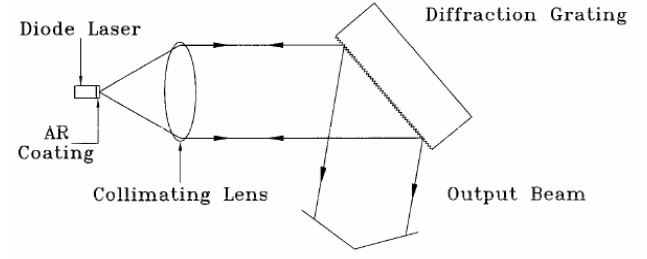
\includegraphics[width=\textwidth]{content/outer_cavity.jpg}
    \caption{Basic configuration of diode laser system with controlled feedback. \cite{Anleitung}}
    \label{fig:cavity}
  \end{figure}

Then the beam hits a diffraction grating. Most of it is directly reflected by the grating, some percent gets reflected back into the laser. Thus forming an external cavity. 

\subsection{Laser Tuning}
The laser tends to lase at the mode frequency with the greatest net gain.
Figure \ref{fig:wavelength} shows different contributions to the net gain. 

\begin{figure}
    \centering
    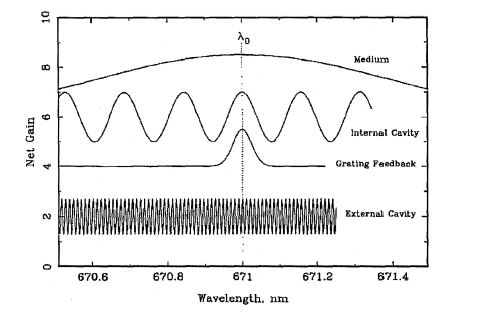
\includegraphics[width=\textwidth]{content/wavelength.jpg}
    \caption{Schematic of the different contributions to the net gain of a laser as a function of frequency. The y-axis is arbitrary, as the curves are displaced for clarity. \cite{Anleitung}}
    \label{fig:wavelength}
  \end{figure}

The frequency of the medium depends mainly on the material properties of the diode. The only tuneable factor is the operation temperature.
The internal cavity can be influenced by modulating the current.
With varying the grating angle the wavelength of the external cavity can be adjusted.

To force the laser into a single mode at a predetermined wavelength $\lambda_0$, each gain from each component should peak at this value. 
Figure \ref{fig:mode} shows the combined grating and external cavity gain overlaid with the internal cavity gain for varied grating angle. In the ideal adjustment the laser oscillates in external mode $e_0$. As the grating angle is changed the gain of this mode is diminished till the laser jumps to other mode with now greater gain.

\begin{figure}
    \centering
    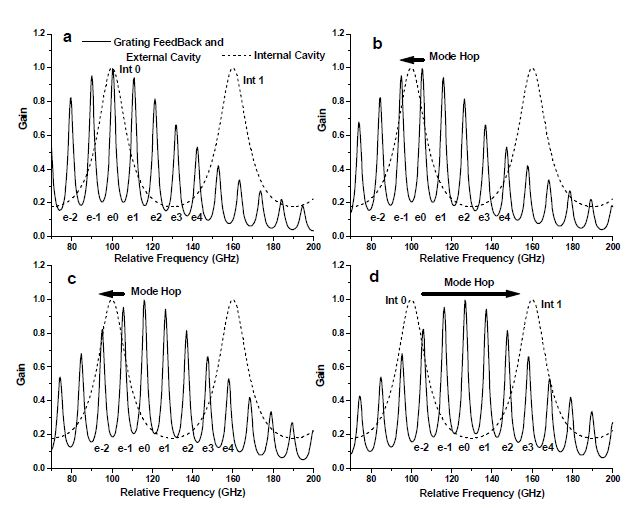
\includegraphics[width=\textwidth]{content/mode.jpg}
    \caption{Series of graphs showing the shift of the  \cite{Anleitung}}
    \label{fig:mode}
  \end{figure}

\subsection{Rubidium absorption spectrum}
\label{sec:rubiAbs}


In the experiment, the absorption spectrum of two isotopes of rubidium is recorded and displayed graphically. 
The closely spaced levels can be seen on the left side of figure \ref{fig:rubiAbs}. The corresponding decays in the power of the transmitted radiation are shown right next to them. They can be related to each other based on the proportionality of frequency and energy.

\begin{figure}[H]
  \centering
  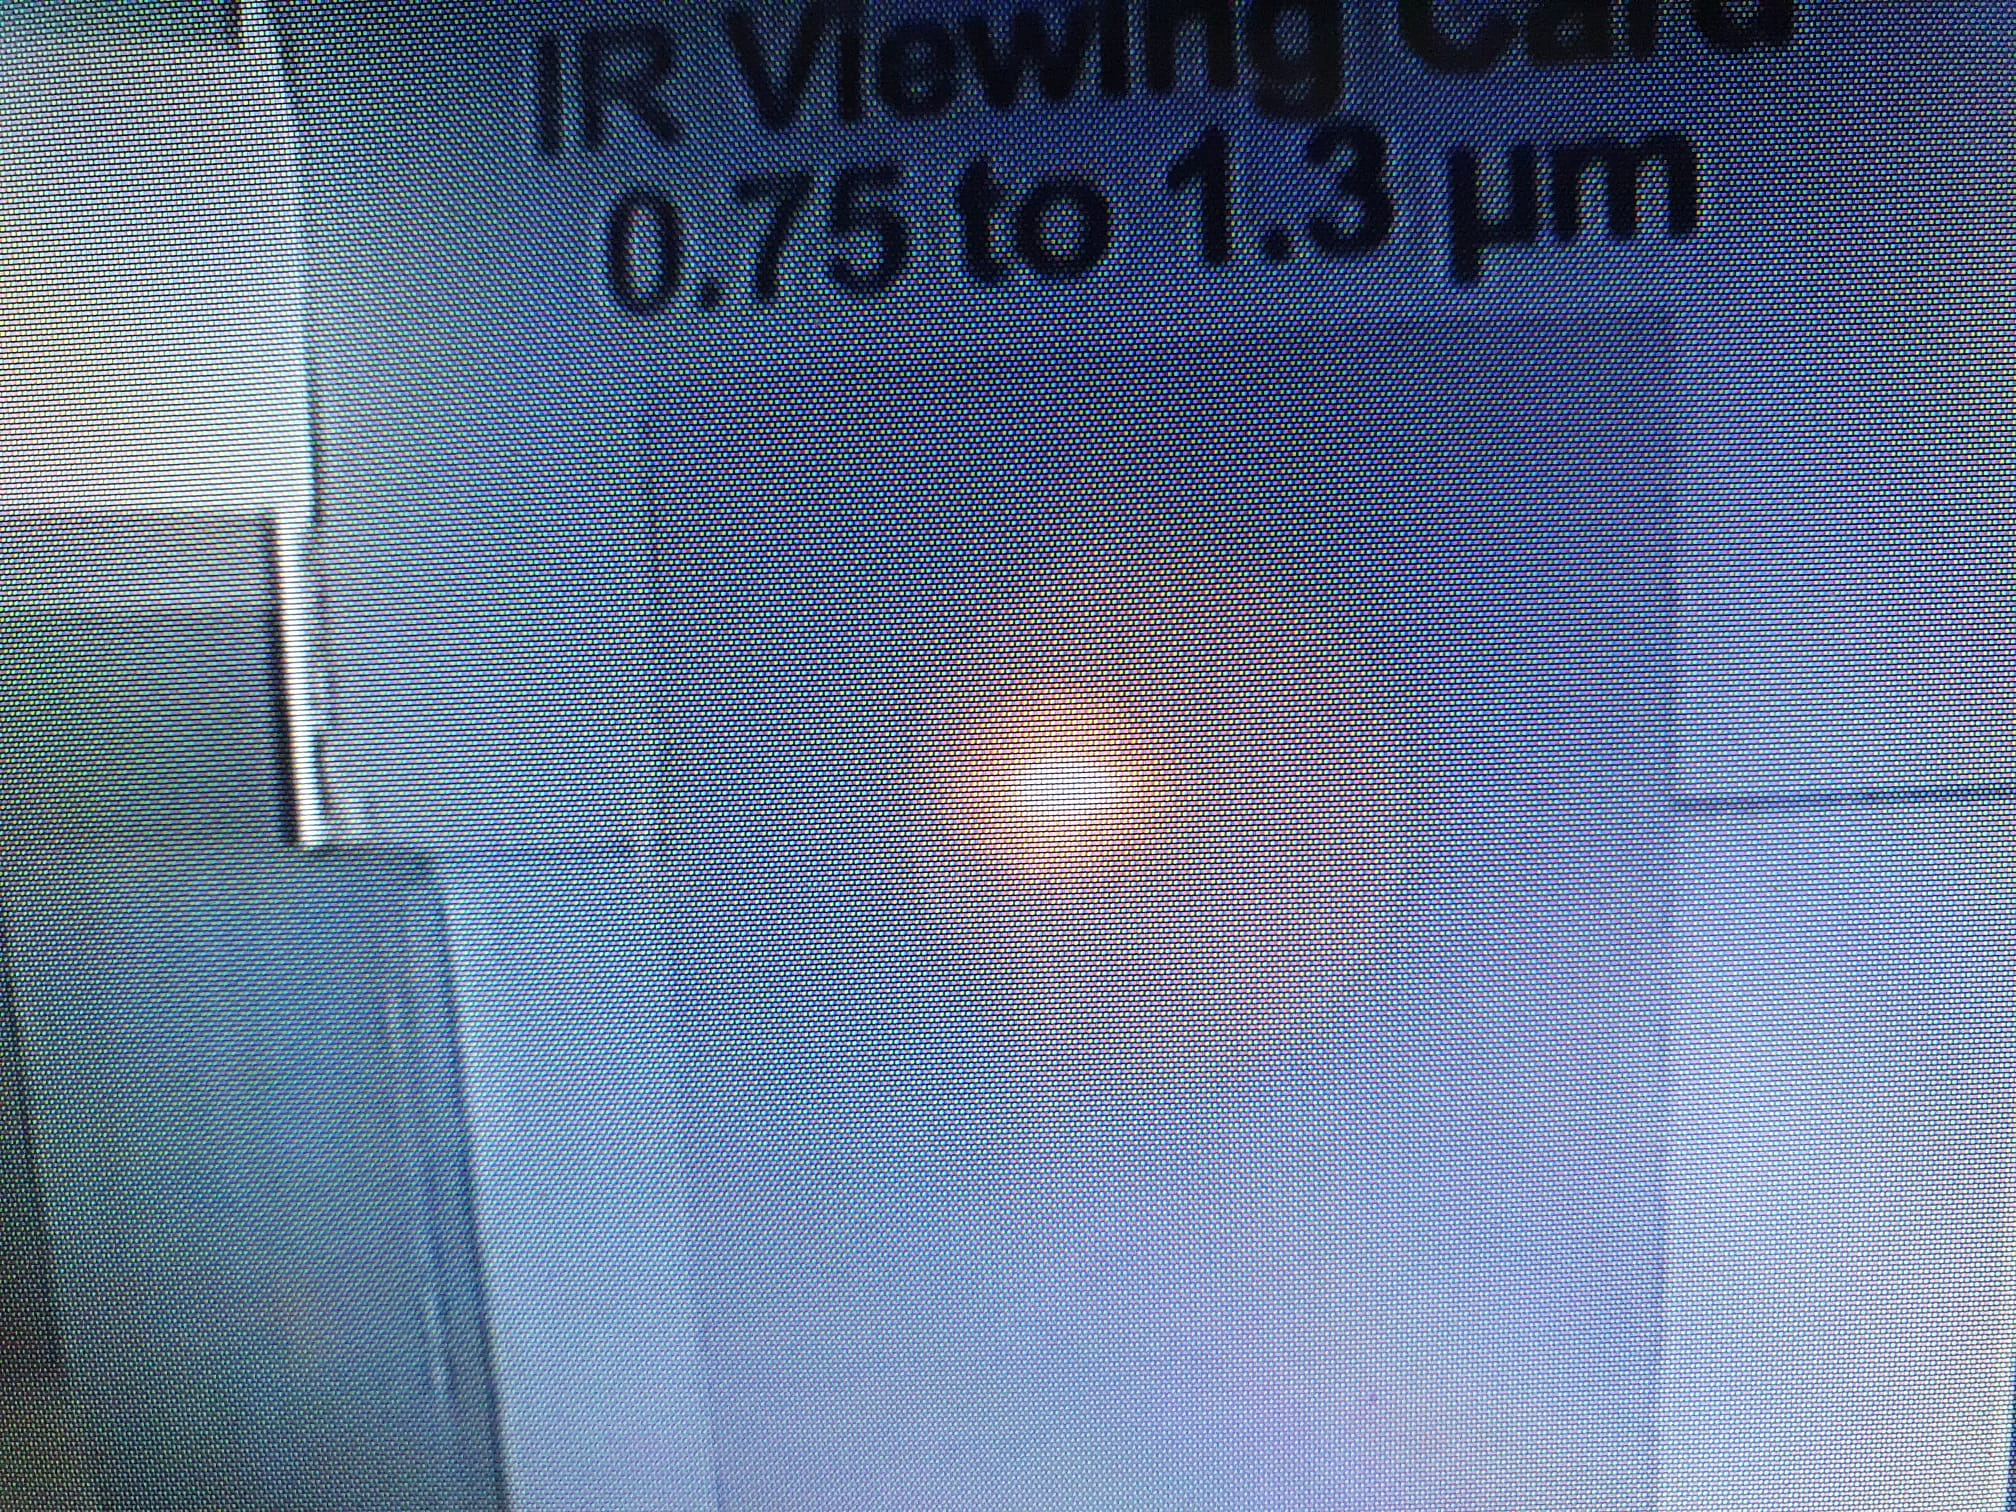
\includegraphics[width=.8\textwidth]{content/led_card.jpeg}
  \caption{The transitions of rubidium, which are made visible in the experiment. \cite{Anleitung}}
  \label{fig:rubiAbs}
\end{figure}